\documentclass[a4paper]{article}

\usepackage[italian]{babel}
\usepackage[utf8]{inputenc}
\usepackage[T1]{fontenc}
\usepackage{enumitem}
\usepackage{graphicx}
\usepackage{float}
\usepackage{longtable}
\usepackage[table]{xcolor}
\usepackage{geometry}

\usepackage{lastpage}
\usepackage[bottom]{footmisc}
\usepackage{fancyhdr}
\usepackage{tabu}

\usepackage{pgffor}
\usepackage{etoolbox}
\usepackage{multirow}



\usepackage[official]{eurosym}

% Navigazione pdf
\usepackage{hyperref}
\hypersetup{
	colorlinks=true,
	linkcolor=black,
	filecolor=magenta,      
	urlcolor=blue,
}

\usepackage{tabularx}

\usepackage{multicol}
\newcommand{\glo}{\textsubscript{\emph{G}}}
\newcommand\hd{\emph{HD Viz}}
\newcommand\cod{\emph{Code of Duty}}
\newcommand{\myparagraph}[1]{\paragraph{#1}\mbox{}\\}
\newcommand{\mysubparagraph}[1]{\subparagraph{#1}\mbox{}\\}

\newcommand{\NdP}{\emph{Norme di Progetto 3.0.0}}
\newcommand{\PdP}{\emph{Piano di Progetto 3.0.0}}
\newcommand{\AdR}{\emph{Analisi dei requisiti 3.0.0}}
\newcommand{\PdQ}{\emph{Piano di Qualifica 3.0.0}}

\definecolor{header}{HTML}{FA8D21}
\definecolor{pari}{HTML}{DBDBDB}
\definecolor{dispari}{HTML}{F5F5F5}

\setcounter{secnumdepth}{4}

\pagestyle{fancy}
\lhead{
\includegraphics[scale=0.06]{../_template/images/logo_crop.png}}

%Titolo del documento
\rhead{\titolodocumento{}}
\cfoot{Pagina \thepage\ di \pageref{LastPage}}
\renewcommand{\footrulewidth}{0.4pt}

\newcommand{\titolodocumento}{Analisi dei requisiti} % Titolo documento
\newcommand{\versione}{ 2.3.0 } % Versione documento
\newcommand{\approvazione}{ Diego Piola } % Responsabile di progetto
\newcommand{\redazione}{\parbox[t]{4cm} {Andrea Mascari\\Damiano Zanardo\\Diego Piola\\}} % Redattori di questo documento
\newcommand{\verifica}{\parbox[t]{4cm} {Andrea Mascari\\Damiano Zanardo \\ Diego Piola \\ Alessandro Flori \\ } } % Verificatori di questo documento
\newcommand{\stato}{In lavorazione} % Approvato 
\newcommand{\uso}{Esterno} % Interno - Esterno
\newcommand{\destinazione}{\parbox[t]{4cm}{Prof Tullio Vardanega \\ Prof. Riccardo Cardin} } % Destinatario ( D1\\D2\\D3 )
\newcommand{\descrizionedocumento}{Il documento elenca casi d'uso e requisiti del progetto } % Descrizione documento

% Mettere sempre la virgola dopo l'ultima riga, se no si rompe la tabella

\def\modifiche{
    {v0.0.1, 02/12/2020, Damiano Zanardo, Analista , Prima bozza{,} aggiunti tutti i capitolati},
}



% Per modificare il frontespizio e diario delle modifiche andare sulla cartella source
% Per aggiungere il contenuto andare sulla cartella source/sections e creare un nuovo file.tex per ogni sezione

% Per parole che devono andare nel glossario aggiungere /glo{} dopo la parola

\begin{document}
    % Frontespizio 
    %\documentclass[a4paper]{article}
%\usepackage[italian]{babel}
\usepackage[utf8]{inputenc}
\usepackage[T1]{fontenc}
\usepackage{enumitem}
\usepackage{graphicx}
\usepackage{float}
\usepackage{longtable}
\usepackage[table]{xcolor}
\usepackage{geometry}

\usepackage{lastpage}
\usepackage[bottom]{footmisc}
\usepackage{fancyhdr}
\usepackage{tabu}

\usepackage{pgffor}
\usepackage{etoolbox}
\usepackage{multirow}



\usepackage[official]{eurosym}

% Navigazione pdf
\usepackage{hyperref}
\hypersetup{
	colorlinks=true,
	linkcolor=black,
	filecolor=magenta,      
	urlcolor=blue,
}

\usepackage{tabularx}

\usepackage{multicol}
%\begin{document}

\begin{titlepage}

	\begin{center}
		
\includegraphics[scale = 0.5]{../_template/images/logo.png}\\
		\large \textbf{Code of Duty - Progetto \emph{HD VIZ}} \\
		\vfill
		\huge \textbf{\titolodocumento}
		\vspace*{\fill}
        
        \vfill
        \large
    \end{center}
    
	\begin{table}[htbp]
        \centering
        \begin{tabular}{r|l}
            \textbf{Versione} & \versione{} \\
            \textbf{Approvazione} & \approvazione{} \\
            \textbf{Redazione} & \redazione{} \\
            \textbf{Verifica} & \verifica{} \\
            \textbf{Stato} & \stato{} \\
            \textbf{Uso} & \uso{} \\
            \textbf{Destinato a} & \destinazione{}
        \end{tabular}
    \end{table}
    
    \begin{center}
        \vfill
        \normalsize
        \textbf{Descrizione}\\
		\descrizionedocumento
        \vfill
        \small
        \texttt{info@codeofduty.it}
	\end{center}
\end{titlepage}

%\end{document}

    
    % Diario delle modifiche
    \newcommand*\mytablecontents{}
\foreach \x [count=\nj] in \modifiche
{
    \foreach \y [count=\ni] in \x
    {
        \ifnum\ni=6
            \xappto\mytablecontents{\y}
            \gappto\mytablecontents{\\}
            \gappto\mytablecontents{\hline}
        \else
            \xappto\mytablecontents{\y&}
        \fi
    }
}

\section*{Diario delle modifiche}

% Impostazioni della tabella
\tabulinesep = 2mm % padding
\taburowcolors [1] 2{pari .. dispari} % colori delle righe
\begin{longtabu} to \textwidth {| X[0.3, c m] | X[0.6,c m] | X[0.7,c m] | X[0.9,c m] | X[0.7,c m] | X[1.2,l m]|} % larghezza delle colonne
\hline
\rowcolor{header} % colore dell'header

\textbf{Ver.} & \textbf{Data} & \textbf{Nominativo} & \textbf{Ruolo} & \textbf{Verificatore} & \multicolumn{1}{c|}{\textbf{Descrizione}}\\
\hline
\mytablecontents

\end{longtabu}

    \pagebreak
    
    % Indice
    \tableofcontents
    \pagebreak
    
    % Se necessari
    % \listoffigures
    % \listoftables
    
    % Contenuto
    \section{Introduzione}
\subsection{Scopo del documento}
	In questo documento vengono illustrate le modilità con cui il gruppo \emph{CODEofDuty} affronterà lo sviluppo del progetto \emph{HDViz}, quali:
	\begin{itemize}
    		\item Analisi dei rischi;
    		\item Presentazione del modello di sviluppo adottato;
    		\item Pianificazione delle attività e divisione dei ruoli;
    		\item Stima dei costi economici e risorse necessarie al compimento del progetto.
	\end{itemize}
\subsection{Scopo del prodotto}
	L'obbiettivo del progetto è quello di creare un'applicazione di visualizzazione di dati con molte dimensioni. L'applicazione dovra permettere diverse visualizzazioni dei dati tramite browser ed è richiesta anche una parte server di supporto che permetta il prelevamento dei dati e la loro elaborazione.
\subsection{Glossario}
	In questo documento vengono definiti e descritti tutti i termini e tecnologie al fine di evitare ambiguità relative al linguaggio utilizzato nei documenti formali. Per facilitare la lettura i termini saranno contrassegnati da una 'G' a pedice.  
\subsection{Riferimenti}
	\subsubsection{Normativi}
	%\subsubsection{Informativi}
    \pagebreak
    \section{Analisi dei rischi}
	Nel corso dello sviluppo di un progetto è naturale incorrere in problemi, tuttavia è possibile evitarne alcuni attraverso l'analisi dei richi. Questa attività è stata effettuata attraverso l'analisi dei principali fattori di rischio. Per ogni fattore di rischio rilevato è stata utilizzata la medesima procedura di identificazionione e risoluzione:
	\begin{enumerate}
		\item \textbf{Individuazione}: Individuazione dei fattori di rischio che rallenterebbero o impedirebbero il proseguimento del progetto;
		\item \textbf{Analisi}: Attività di studio dei fattori di rischio, ad ognuno di essi è stata assegnata una probabilità che si verifichi e un indice di gravità, basato sull'impatto che potrebbe avere sul progetto;
		\item \textbf{Pianificazione di Controllo}: Studio di un metodologia per evitare il verificarsi di un determinato fattore di rischio e un piano di risoluzione nel caso essa si verifichi;
		\item \textbf{Monitoraggio}: I fattori di rischio vanno tenuti sotto constante controllo, cercando di evitare che si verifichino se possibile oppure agire tempestivamente per minimizzare i danni;
	\end{enumerate}
	Ogni fattore di rischio rilevato è stato definito e raggruppato secondo varie tipologie:
	\begin{itemize}
		\item \textbf{RT}: Rischio Tecnologici;
		\item \textbf{RO}: Rischi Organizzativi;
		\item \textbf{RI}: Rischi Interpersonali;
	\end{itemize}
	\subsection{Rischi Tecnologici}
	\def\productquality{
    		{
        		Inesperienza
			Tecnologica
			RT1,
        		La maggior parte delle tecnologie richieste nello sviluppo del progetto sono nuove per molti componenti del team, 
        		Il responsabile dovrà rilevare conoscenze e lacune dei vari componenti del team provando ad indicare una via ottimale per risolvere la mancanza di conoscenze,
        		Occorrenza: Alta 
			Pericolosità: Alta,
        		I compiti più onerasi verranno assegnati a più persone favorendo l'assistenza reciproca
    		},
	}
	\newcommand*\metricstable{}
\foreach \x [count=\nj] in \productquality
{
    \foreach \y [count=\ni] in \x
    {
        \ifnum\ni=4
            \xappto\metricstable{\y}
            \gappto\metricstable{\\}
            \gappto\metricstable{\hline}
        \else\ifnum\ni=5
            \xappto\metricstable{\noexpand\multicolumn{4}{| l |}{NOTE: \y}}
            \gappto\metricstable{\\}
            \gappto\metricstable{\hline}
        \else
            \xappto\metricstable{\y&}
        \fi\fi
    }
}

% Impostazioni della tabella
\tabulinesep = 2mm % padding
\taburowcolors [1] 2{pari .. dispari} % colori delle righe
\begin{longtabu} to \textwidth {| X[0.7,c m] | X[0.7,c m] | X[0.4,c m] | X[0.4,c m]|} % larghezza delle colonne
\hline
\rowcolor{header} % colore dell'header

\textbf{Nome} & \textbf{Formula} & \textbf{Valore sufficiente} & \textbf{Valore ottimo}\\
\hline
\metricstable

\end{longtabu}

\undef\metricstable{}
	\pagebreak
	\subsection{Rischi Organizzativi}

		\def\productquality{
    			{
        			Calcolo
				Tempistiche e Costi
				RO1,
        			Causa RT1 le valutazioni sulle tempistiche e i costi economici potrebbero essere imprecisi, 
        			Vengono predisposte delle tabelle sulle tempistiche e sarà compito del responsabile monitorare l'andamento dello sviluppo,
        			Occorrenza: Alta 
				Pericolosità: Alta,
        			Il responsabile provvederà all'assegnazione di maggiori risorse
    			},
		}
		\newcommand*\metricstable{}
\foreach \x [count=\nj] in \productquality
{
    \foreach \y [count=\ni] in \x
    {
        \ifnum\ni=4
            \xappto\metricstable{\y}
            \gappto\metricstable{\\}
            \gappto\metricstable{\hline}
        \else\ifnum\ni=5
            \xappto\metricstable{\noexpand\multicolumn{4}{| l |}{NOTE: \y}}
            \gappto\metricstable{\\}
            \gappto\metricstable{\hline}
        \else
            \xappto\metricstable{\y&}
        \fi\fi
    }
}

% Impostazioni della tabella
\tabulinesep = 2mm % padding
\taburowcolors [1] 2{pari .. dispari} % colori delle righe
\begin{longtabu} to \textwidth {| X[0.7,c m] | X[0.7,c m] | X[0.4,c m] | X[0.4,c m]|} % larghezza delle colonne
\hline
\rowcolor{header} % colore dell'header

\textbf{Nome} & \textbf{Formula} & \textbf{Valore sufficiente} & \textbf{Valore ottimo}\\
\hline
\metricstable

\end{longtabu}

\undef\metricstable{}

		\def\productquality{
			{
        			Impegni
				Accademici
				RO2,
        			Il periodo di sviluppo del progetto inizia a ridosso della sessione d'esami universitaria a cui tutti i membri del gruppo si vedono impegnati in diverse occasioni, 
        			In sede di riunione il team ha deciso di condividere i periodi di tempo in cui il loro contributo al progetto potrebbe calare o venir meno,
        			Occorrenza: Media 
				Pericolosità: Media,
        			Il lavoro verrà assegnato nel rispetto degli altri impegni accademici
    			},
		}
		\newcommand*\metricstable{}
\foreach \x [count=\nj] in \productquality
{
    \foreach \y [count=\ni] in \x
    {
        \ifnum\ni=4
            \xappto\metricstable{\y}
            \gappto\metricstable{\\}
            \gappto\metricstable{\hline}
        \else\ifnum\ni=5
            \xappto\metricstable{\noexpand\multicolumn{4}{| l |}{NOTE: \y}}
            \gappto\metricstable{\\}
            \gappto\metricstable{\hline}
        \else
            \xappto\metricstable{\y&}
        \fi\fi
    }
}

% Impostazioni della tabella
\tabulinesep = 2mm % padding
\taburowcolors [1] 2{pari .. dispari} % colori delle righe
\begin{longtabu} to \textwidth {| X[0.7,c m] | X[0.7,c m] | X[0.4,c m] | X[0.4,c m]|} % larghezza delle colonne
\hline
\rowcolor{header} % colore dell'header

\textbf{Nome} & \textbf{Formula} & \textbf{Valore sufficiente} & \textbf{Valore ottimo}\\
\hline
\metricstable

\end{longtabu}

\undef\metricstable{}

		\def\productquality{
			{
        			Impegni
				Personali
				RO3,
        			è possibile il verificarsi di imprevisti personali che potrebbero influire nel corretto sviluppo del progetto, 
        			è compito di ogni membro del gruppo segnalare un eventuale imprevisto al responsabile del gruppo in modo da permettergli di riorganizzare l'agenda,
        			Occorrenza: Bassa 
				Pericolosità: Bassa,
        			Il responsabile riallocherà risorse al fine di evitare ritardi
    			},
		}
		\newcommand*\metricstable{}
\foreach \x [count=\nj] in \productquality
{
    \foreach \y [count=\ni] in \x
    {
        \ifnum\ni=4
            \xappto\metricstable{\y}
            \gappto\metricstable{\\}
            \gappto\metricstable{\hline}
        \else\ifnum\ni=5
            \xappto\metricstable{\noexpand\multicolumn{4}{| l |}{NOTE: \y}}
            \gappto\metricstable{\\}
            \gappto\metricstable{\hline}
        \else
            \xappto\metricstable{\y&}
        \fi\fi
    }
}

% Impostazioni della tabella
\tabulinesep = 2mm % padding
\taburowcolors [1] 2{pari .. dispari} % colori delle righe
\begin{longtabu} to \textwidth {| X[0.7,c m] | X[0.7,c m] | X[0.4,c m] | X[0.4,c m]|} % larghezza delle colonne
\hline
\rowcolor{header} % colore dell'header

\textbf{Nome} & \textbf{Formula} & \textbf{Valore sufficiente} & \textbf{Valore ottimo}\\
\hline
\metricstable

\end{longtabu}

\undef\metricstable{}


	\subsection{Rischi Interpersonali}
		\def\productquality{
			{
        			Irreperibilita
				momentanea
				RI1,
        			Potrebbero verificarsi momenti in cui uno o più membri del team siano irreperibili, 
        			è responsabilità di ogni membro del gruppo comunicare eventuali imprevisti e organizzarsi in modo da non ostacolare il calendario delle consegne,
        			Occorrenza: Bassa 
				Pericolosità: Media,
        			Abbiamo a disposizione diversi mezzi di comunicazione dove comunicare eventuali problematiche
    			},
		}
		\newcommand*\metricstable{}
\foreach \x [count=\nj] in \productquality
{
    \foreach \y [count=\ni] in \x
    {
        \ifnum\ni=4
            \xappto\metricstable{\y}
            \gappto\metricstable{\\}
            \gappto\metricstable{\hline}
        \else\ifnum\ni=5
            \xappto\metricstable{\noexpand\multicolumn{4}{| l |}{NOTE: \y}}
            \gappto\metricstable{\\}
            \gappto\metricstable{\hline}
        \else
            \xappto\metricstable{\y&}
        \fi\fi
    }
}

% Impostazioni della tabella
\tabulinesep = 2mm % padding
\taburowcolors [1] 2{pari .. dispari} % colori delle righe
\begin{longtabu} to \textwidth {| X[0.7,c m] | X[0.7,c m] | X[0.4,c m] | X[0.4,c m]|} % larghezza delle colonne
\hline
\rowcolor{header} % colore dell'header

\textbf{Nome} & \textbf{Formula} & \textbf{Valore sufficiente} & \textbf{Valore ottimo}\\
\hline
\metricstable

\end{longtabu}

\undef\metricstable{}
		\def\productquality{
			{
        			Contrasti 
				interni
				RI2,
        			Potrebbero verificarsi divergenze tra i membri del gruppo, 
        			Ciascun dei membri del team si impegna ad agire al fine di non ostacolare il naturale svolgimento del progetto e discutere di eventuali problemi solo in seduta di riunione,
        			Occorrenza: Bassa 
				Pericolosità: Media,
        			Il responsabile avrà il compito di fare da mediatore in caso ci fossero contrasti tra i membri del gruppo
    			},
		}
		\newcommand*\metricstable{}
\foreach \x [count=\nj] in \productquality
{
    \foreach \y [count=\ni] in \x
    {
        \ifnum\ni=4
            \xappto\metricstable{\y}
            \gappto\metricstable{\\}
            \gappto\metricstable{\hline}
        \else\ifnum\ni=5
            \xappto\metricstable{\noexpand\multicolumn{4}{| l |}{NOTE: \y}}
            \gappto\metricstable{\\}
            \gappto\metricstable{\hline}
        \else
            \xappto\metricstable{\y&}
        \fi\fi
    }
}

% Impostazioni della tabella
\tabulinesep = 2mm % padding
\taburowcolors [1] 2{pari .. dispari} % colori delle righe
\begin{longtabu} to \textwidth {| X[0.7,c m] | X[0.7,c m] | X[0.4,c m] | X[0.4,c m]|} % larghezza delle colonne
\hline
\rowcolor{header} % colore dell'header

\textbf{Nome} & \textbf{Formula} & \textbf{Valore sufficiente} & \textbf{Valore ottimo}\\
\hline
\metricstable

\end{longtabu}

\undef\metricstable{}
	\subsection{Rischi legati al lavoro a distanza}
		 
    \pagebreak
    \section{Pianificazione}
	Alla luce delle scadenze riportate nella sezione 1.5 e alle scadenze interne si è deciso di dividere il progetto in cinque fasi:
	\begin{itemize}
		\item \textbf{Analisi};
		\item \textbf{Consolidamento dei requisiti};
		\item \textbf{Progettazione architetturale};
		\item \textbf{Progettazione di dettaglio e codifica};
		\item \textbf{Validazione e collaudo}.
	\end{itemize}
	Ognuna di queste cinque fasi sarà formata da diverse sottoattività mostrate nel corrispettivo diagramma di Gantt.

	\subsection{Analisi}
	\textbf{Periodo}: dal 26-11-2020 al 10-01-2021 \\
	La fase di Analisi è composta da sei attività che corrispondono alla produzione dei relativi documenti:
	\begin{itemize}
		\item \textbf{Studio di fattibilità}: Ogni capitolato proposto viene analizzato e discusso con i membri del gruppo. Ogni capitolato viene poi classificato in base alle preferenze e ai punti di iteresse riscontrati. Il capitolato che avrà riscosso più preferenze viene scelto come capitolato effetivo;
		\item \textbf{Norme di progetto}: Vengono definite le regole che il team dovrà rispettare durante lo sviluppo del progetto;
		\item \textbf{Piano di Progetto}: Si analizzato le attività, i compiti e le risorse che verranno distribuite tra i membri del team, presenta il calcolo del preventivo per la realizzazione del progetto;
		\item \textbf{Analisi dei requisiti}: Vengono studiati e analizzati i requisiti del capitolato scelto ( \textbf{C4} ) nello studio di fattibilità;
		\item \textbf{Piano di qualifica}: Durante questa attività si individuano le metodologie da usare per garantire la qualità del prodotto;
		\item \textbf{Glossario}: Questo documento viene redatto per definire la terminologia usata al fine di evitare ambiguità;
	\end{itemize}
	\subsubsection{Diagramma}
		\begin{figure}[H]
        		\centering
        		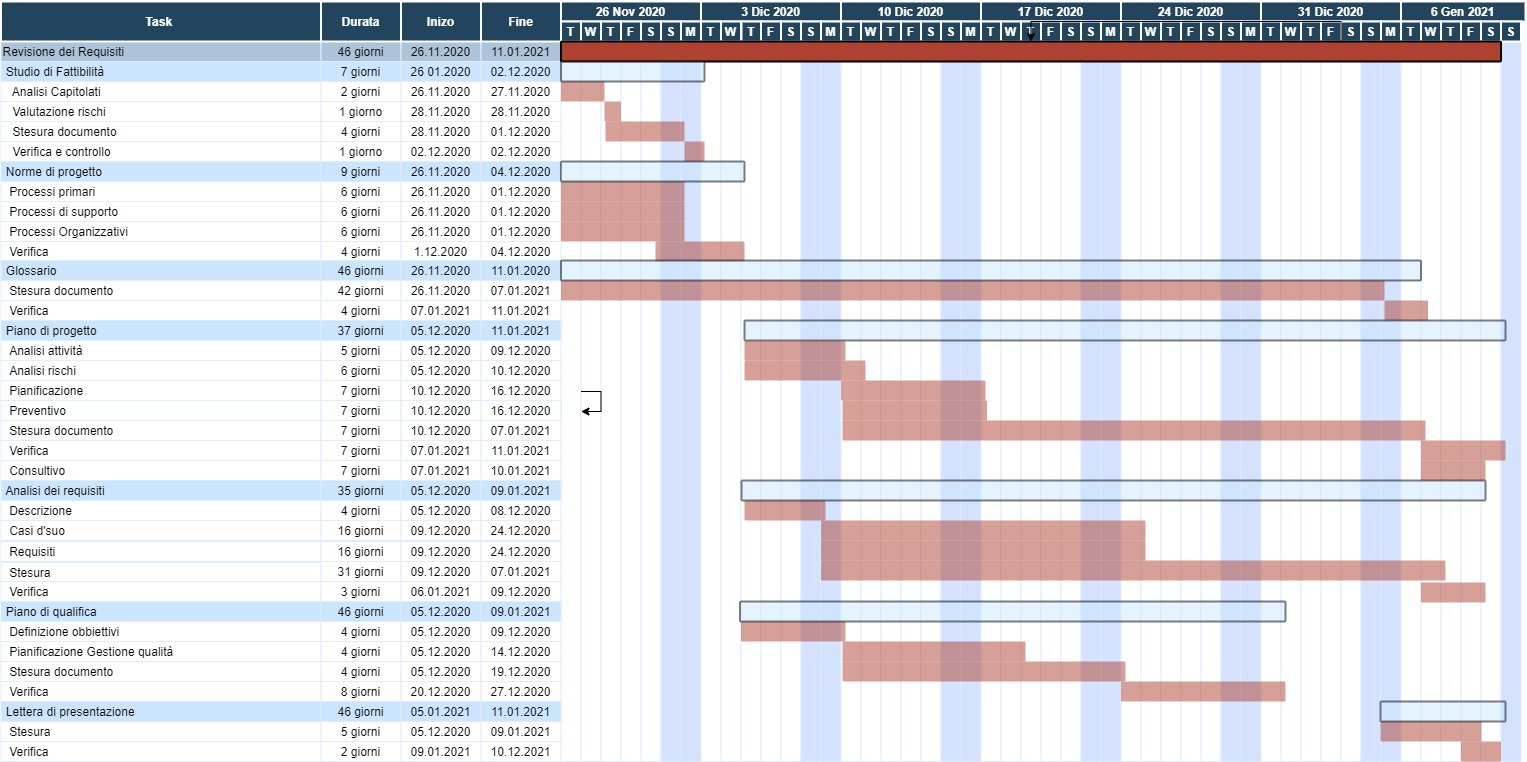
\includegraphics[width=0.8\textwidth]{source/img/analisiattivita.jpg}
        		\caption{Divisione oraria dell'attività di analisi}
    		\end{figure}

	\subsection{Consolidamento dei requisiti}
	\textbf{Periodo}: dal 12-01-2021 al 18-01-2021 \\
	La fase di consolidamento dei requisiti è intermedia tra la fine della'attività di Analisi e il giorno della presentazione della Revisione dei Requisiti. \\
	Durante la seguente fase si svolgeranno attività di consolidamento dei requisiti osservati nella fase precedente e verrà preparata la presentazione per la Revisione dei Requisiti.
	
	\subsubsection{Diagramma}
		\begin{figure}[H]
        		\centering
        		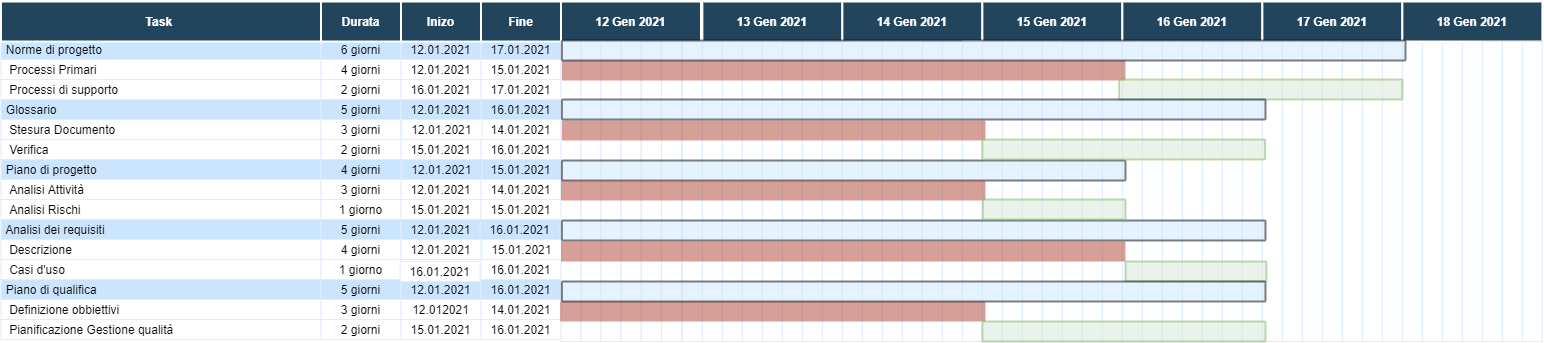
\includegraphics[width=0.8\textwidth]{source/img/Consolidamento_Requisiti.png}
        		\caption{Divisione oraria dell'attività di analisi}
    		\end{figure}
	
	\subsection{Progettazione architetturale}
	\textbf{Periodo}: dal 19-01-2021 al 01-03-2021
	Successivamente alla presentazione della Revisione dei Requisiti inizia la fase di progettazione architetturare che terminera con la consegna della Revisione di Progettazione, lo scopo di questo periodo è l'individuazione di una soluzione architetturale che soddisfi i seguenti requisiti:
	\begin{itemize}
		\item \textbf{Technology Baseline}: verrà stilato l'allegato tecnico nel quale verranno individuati i design pattern che verranno adottati nello sviluppo del progetto. Inoltre verrà redatto il Proof Of Concept da consegnare al committente;
		\item \textbf{Incremento e verifica}: Se necessarrio vengono migliorati i documenti consegnati durante la fase iniziale.
	\end{itemize}
	
	\subsubsection{Diagramma}
		\begin{figure}[H]
        		\centering
        		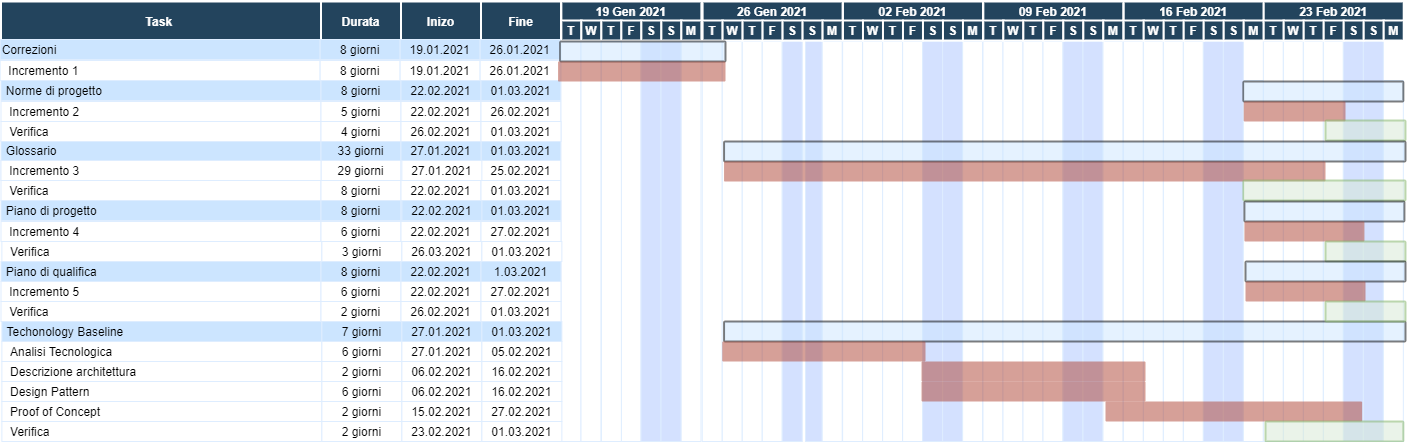
\includegraphics[width=0.8\textwidth]{source/img/Progettazione_architetturale.png}
        		\caption{Divisione oraria dell'attività di analisi}
    		\end{figure}
	
	\subsection{Progettazione di dettaglio e codifica}
	\textbf{Periodo}: dal 02-03-2021 al 02-04-2021
	Col termine della Revisione di Progettazione, inizia la fase di progettazione di dettaglio e codifica e terminerà con la Revisione di Qualifica, la seguente fase è composta da nuovi incrementi e attività:
	\begin{itemize}
		\item \textbf{Incremento e verifica}: Se necessario verranno migliorati i documenti consegnati durante la fase precedente;
		\item \textbf{Product Baseline}: Vengono studiati i design pattern, classi e attività necessarie alla codifica;
		\item \textbf{Specifica Tecnica}: Realizzazione di un documento contenente le specifiche del prodotto motivandone la scelta;
		\item \textbf{Codifica}
		\item \textbf{Manuale Utente}: Redazione del manuale utente del prodotto.
	\end{itemize}
	
	\subsubsection{Diagramma}
		\begin{figure}[H]
        		\centering
        		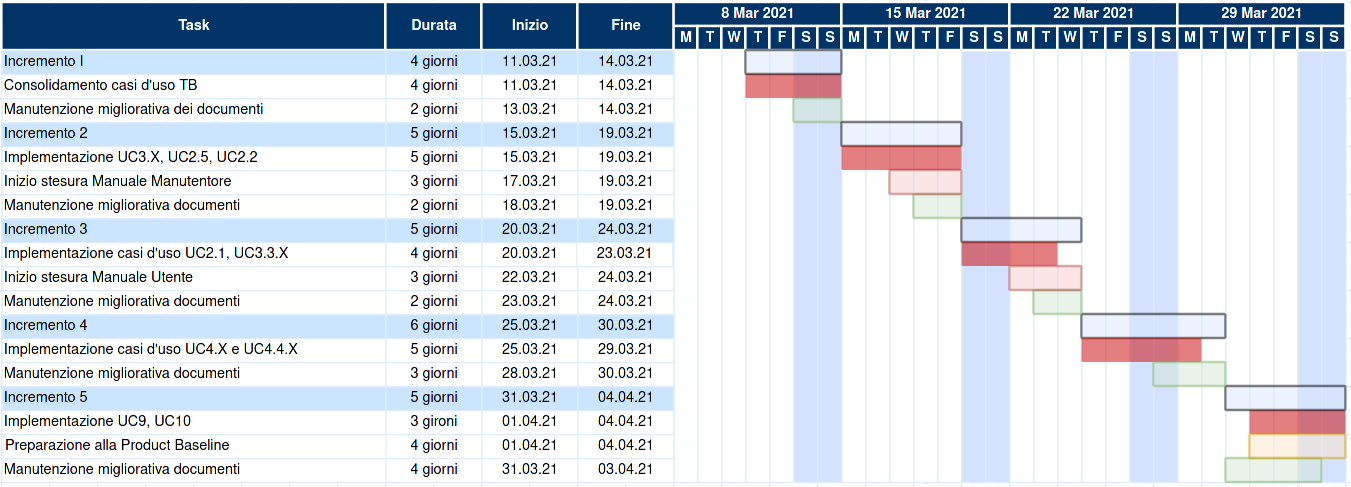
\includegraphics[width=0.8\textwidth]{source/img/Progettazionedettaglio_codifica.png}
        		\caption{Divisione oraria dell'attività di analisi}
    		\end{figure}

	\subsection{Validazione e Collaudo}
	\textbf{Periodo}: dal 03-03-2021 al 03-04-2021
	Ultima fase del progetto che terminerà con la Revisione di Accettazione, la seguente fase è composta da incrementi e nuove attività da svolgere:
	\begin{itemize}
		\item \textbf{Incremento e verifica}: Se necessario verranno migliorati i documenti consegnati durante la fase precedente;
		\item \textbf{Validazione e Collaudo}: Si eseguono i test finali di collaudo dell'applicazione nella sua interezza.
	\end{itemize}
	
	\subsubsection{Diagramma}
    \pagebreak
    \section{Preventivo}
Nel Preventivo è indicata la divisione delle ore per ogni fase individuata nella sezione 4 del presente documento, insieme al prospetto economico. All'interno del Riepilogo è presentato il costo totale preventivato. Il tutto è corredato da diagrammi esemplificativi.
Si noti che nelle tabelle sono state utilizzate delle sigle, definite nelle \NdP . % mi porto avanti con le versioni
\subsection{Analisi}

    \subsubsection{Prospetto orario}
    %startTable
    \def\hourlycontent{
        {Andrea Breggion,6,14,3,0,0,6,29},
        {Matteo Falsetti,0,5,3,10,0,11,29},
        {Alessandro Flori,2,4,3,8,0,12,29},
        {Andrea Mascari,0,0,14,2,0,13,29},
        {Diego Piola,6,13,3,0,0,7,29},
        {Andrea Signori,12,6,4,0,0,7,29},
        {Damiano Zanardo,0,7,14,0,0,8,29},
        {Ore totali, 25, 51, 44, 19, 0, 64, 203},
    }
    %endTable
    \newcommand*\hourlysummary{}
\foreach \x [count=\nj] in \hourlycontent
{
    \foreach \y [count=\ni] in \x
    {
        \ifnum\ni=8
            \xappto\hourlysummary{\y}
            \gappto\hourlysummary{\\}
            \gappto\hourlysummary{\hline}
        \else
            \xappto\hourlysummary{\y&}
        \fi
    }
}

% Impostazioni della tabella
\tabulinesep = 2mm % padding
\taburowcolors [1] 2{pari .. dispari} % colori delle righe
\begin{longtabu} to \textwidth {| X[0.3, c m] | X[0.1, c m] | X[0.1, c m] | X[0.1, c m] | X[0.1, c m] | X[0.1, c m] | X[0.1, c m] | X[0.1, c m] |}
\hline
\rowcolor{header} % colore dell'header
\textbf{Membro} &
\textbf{Re} & 
\textbf{Ad} & 
\textbf{An} & 
\textbf{Pt} & 
\textbf{Pr} & 
\textbf{Ve} & 
\textbf{Ore totali} \\
\hline
\hourlysummary
\end{longtabu}
\undef\hourlysummary{}
    \begin{figure}[H]
        \centering
        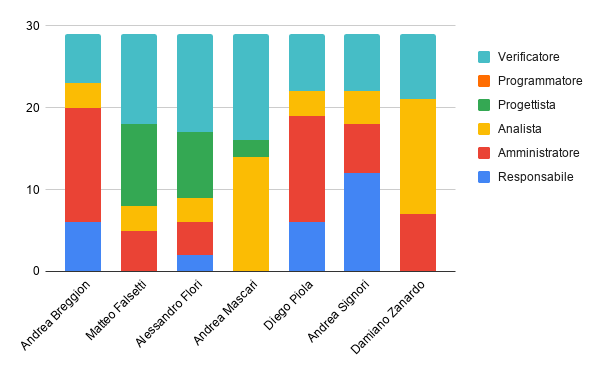
\includegraphics[width=0.8\textwidth]{source/img/analisi_orari.png}
        \caption{Divisione oraria dell'attività di analisi}
    \end{figure}
    \subsubsection{Prospetto economico}
    %startTable
    \def\salarycontent{
        {Amministratore,49,20,980},
        {Analista,44,25,1100},
        {Progettista,20,22,440},
        {Programmatore,0,15,0},
        {Responsabile,26,30,780},
        {Verificatore,64,15,960},
        {Totale,203,127,4260},
    }
    %endTable
    \newcommand*\salarysummary{}
\foreach \x [count=\nj] in \salarycontent
{
    \foreach \y [count=\ni] in \x
    {
        \ifnum\ni=1
            \xappto\salarysummary{\noexpand\textbf{\y}&}
        \else\ifnum\ni=3
            \xappto\salarysummary{\noexpand\euro\ \y&}
        \else\ifnum\ni=4
            \xappto\salarysummary{\noexpand\euro\ \y}
            \gappto\salarysummary{\\}
            \gappto\salarysummary{\hline} 
        \else
            \xappto\salarysummary{\y&}
        \fi\fi\fi
    }
}

% Impostazioni della tabella
\tabulinesep = 2mm % padding
\taburowcolors [1] 2{pari .. dispari} % colori delle righe
\begin{longtabu} to \textwidth {| X[0.1, c m] | X[0.1, c m] | X[0.1, c m] | X[0.1, c m] |}
\hline
\rowcolor{header} % colore dell'header
\textbf{Ruolo} &
\textbf{Ore} &
\textbf{Costo unitario (€)} & 
\textbf{Costo totale (€)} \\
\hline
\salarysummary
\end{longtabu}
\undef\salarysummary
    \begin{figure}[H]
        \centering
        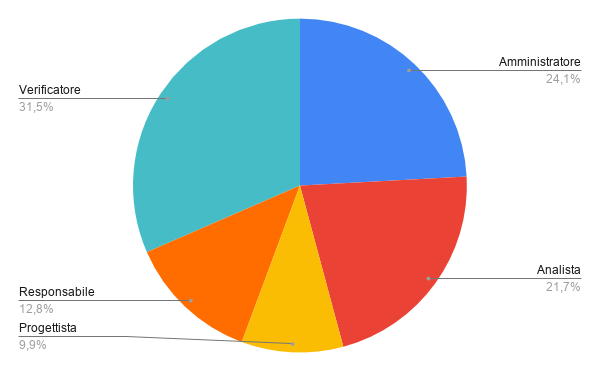
\includegraphics[width=0.8\textwidth]{source/img/analisi_ruoli.png}
        \caption{costo del personale nella fase di analisi}
    \end{figure}
\subsection{Consolidamento dei requisiti}
    \subsubsection{Prospetto orario}
    %startTable
    \def\hourlycontent{
        {Andrea Breggion,0,3,0,0,0,2,5},
        {Matteo Falsetti,0,0,0,1,0,4,5},
        {Alessandro Flori,0,0,0,1,0,4,5},
        {Andrea Mascari,0,0,5,0,0,0,5},
        {Diego Piola,2,0,3,0,0,0,5},
        {Andrea Signori,0,0,2,0,0,3,5},
        {Damiano Zanardo,0,0,5,0,0,0,5},
        {Ore totali,2,3,15,2,0,13,35},
    }
    %endTable
    \newcommand*\hourlysummary{}
\foreach \x [count=\nj] in \hourlycontent
{
    \foreach \y [count=\ni] in \x
    {
        \ifnum\ni=8
            \xappto\hourlysummary{\y}
            \gappto\hourlysummary{\\}
            \gappto\hourlysummary{\hline}
        \else
            \xappto\hourlysummary{\y&}
        \fi
    }
}

% Impostazioni della tabella
\tabulinesep = 2mm % padding
\taburowcolors [1] 2{pari .. dispari} % colori delle righe
\begin{longtabu} to \textwidth {| X[0.3, c m] | X[0.1, c m] | X[0.1, c m] | X[0.1, c m] | X[0.1, c m] | X[0.1, c m] | X[0.1, c m] | X[0.1, c m] |}
\hline
\rowcolor{header} % colore dell'header
\textbf{Membro} &
\textbf{Re} & 
\textbf{Ad} & 
\textbf{An} & 
\textbf{Pt} & 
\textbf{Pr} & 
\textbf{Ve} & 
\textbf{Ore totali} \\
\hline
\hourlysummary
\end{longtabu}
\undef\hourlysummary{} 
    \begin{figure}[H]
        \centering
        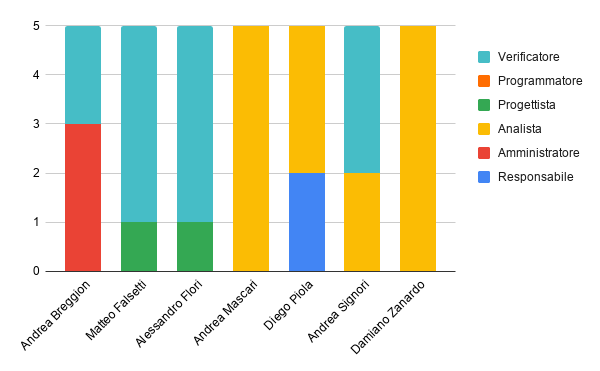
\includegraphics[width=0.8\textwidth]{source/img/consolidamento_orari.png}
        \caption{divisione oraria dell'attività di consolidamento dei requisiti}
    \end{figure}
    \subsubsection{Prospetto economico}
    %startTable
    \def\salarycontent{
        {Amministratore,3,20,60},
        {Analista,15,25,375},
        {Progettista,2,22,44},
        {Programmatore,0,15,0},
        {Responsabile,2,30,60},
        {Verificatore,13,15,195},
        {Totale,35,127,734},
    }
    %endTable
    \newcommand*\salarysummary{}
\foreach \x [count=\nj] in \salarycontent
{
    \foreach \y [count=\ni] in \x
    {
        \ifnum\ni=1
            \xappto\salarysummary{\noexpand\textbf{\y}&}
        \else\ifnum\ni=3
            \xappto\salarysummary{\noexpand\euro\ \y&}
        \else\ifnum\ni=4
            \xappto\salarysummary{\noexpand\euro\ \y}
            \gappto\salarysummary{\\}
            \gappto\salarysummary{\hline} 
        \else
            \xappto\salarysummary{\y&}
        \fi\fi\fi
    }
}

% Impostazioni della tabella
\tabulinesep = 2mm % padding
\taburowcolors [1] 2{pari .. dispari} % colori delle righe
\begin{longtabu} to \textwidth {| X[0.1, c m] | X[0.1, c m] | X[0.1, c m] | X[0.1, c m] |}
\hline
\rowcolor{header} % colore dell'header
\textbf{Ruolo} &
\textbf{Ore} &
\textbf{Costo unitario (€)} & 
\textbf{Costo totale (€)} \\
\hline
\salarysummary
\end{longtabu}
\undef\salarysummary
    \begin{figure}[H]
        \centering
        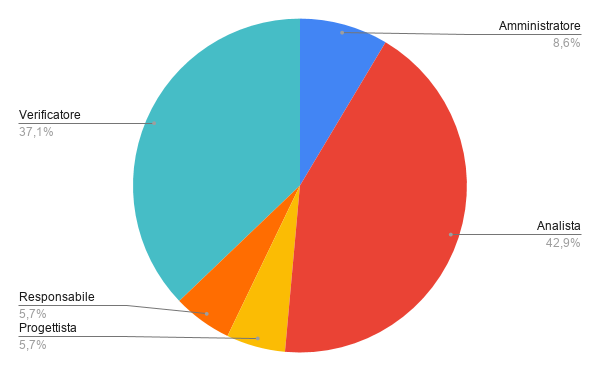
\includegraphics[width=0.8\textwidth]{source/img/consolidamento_ruoli.png}
        \caption{costo del personale nella fase di consolidamento dei requisiti}
    \end{figure}
\subsection{Progettazione architetturale}
    \subsubsection{Prospetto orario}
    %startTable
    \def\hourlycontent{
        {Andrea Breggion,0,7,4,6,5,4,26},
        {Matteo Falsetti,0,0,5,7,0,14,26},
        {Alessandro Flori,0,0,7,10,0,9,26},
        {Andrea Mascari,4,0,0,11,6,5,26},
        {Diego Piola,5,0,6,9,6,0,26},
        {Andrea Signori,0,6,4,7,5,4,26},
        {Damiano Zanardo,0,0,0,12,9,5,26},
        {Ore totali, 9, 13, 26, 62, 31, 41, 182},
    }
    %endTable
    \newcommand*\hourlysummary{}
\foreach \x [count=\nj] in \hourlycontent
{
    \foreach \y [count=\ni] in \x
    {
        \ifnum\ni=8
            \xappto\hourlysummary{\y}
            \gappto\hourlysummary{\\}
            \gappto\hourlysummary{\hline}
        \else
            \xappto\hourlysummary{\y&}
        \fi
    }
}

% Impostazioni della tabella
\tabulinesep = 2mm % padding
\taburowcolors [1] 2{pari .. dispari} % colori delle righe
\begin{longtabu} to \textwidth {| X[0.3, c m] | X[0.1, c m] | X[0.1, c m] | X[0.1, c m] | X[0.1, c m] | X[0.1, c m] | X[0.1, c m] | X[0.1, c m] |}
\hline
\rowcolor{header} % colore dell'header
\textbf{Membro} &
\textbf{Re} & 
\textbf{Ad} & 
\textbf{An} & 
\textbf{Pt} & 
\textbf{Pr} & 
\textbf{Ve} & 
\textbf{Ore totali} \\
\hline
\hourlysummary
\end{longtabu}
\undef\hourlysummary{}
    \begin{figure}[H]
        \centering
        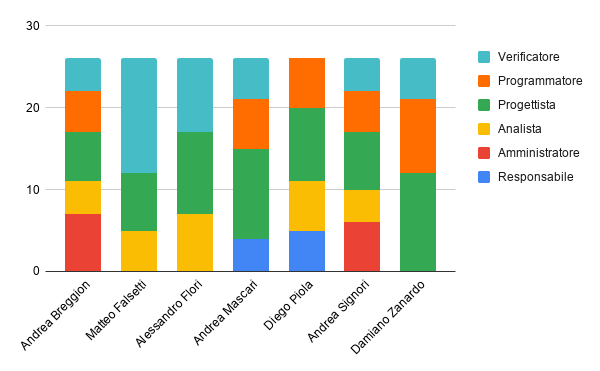
\includegraphics[width=0.8\textwidth]{source/img/architettura_orari.png}
        \caption{divisione oraria dell'attività di progettazione architetturale}
    \end{figure}
    \subsubsection{Prospetto economico}
    %startTable
    \def\salarycontent{
        {Amministratore,13,20,260},
        {Analista,26,25,650},
        {Progettista,62,22,1364},
        {Programmatore,31,15,465},
        {Responsabile,31,15,465},
        {Verificatore,41,15,615},
        {Totale,182,127,3624},
    }
    %endTable
    \newcommand*\salarysummary{}
\foreach \x [count=\nj] in \salarycontent
{
    \foreach \y [count=\ni] in \x
    {
        \ifnum\ni=1
            \xappto\salarysummary{\noexpand\textbf{\y}&}
        \else\ifnum\ni=3
            \xappto\salarysummary{\noexpand\euro\ \y&}
        \else\ifnum\ni=4
            \xappto\salarysummary{\noexpand\euro\ \y}
            \gappto\salarysummary{\\}
            \gappto\salarysummary{\hline} 
        \else
            \xappto\salarysummary{\y&}
        \fi\fi\fi
    }
}

% Impostazioni della tabella
\tabulinesep = 2mm % padding
\taburowcolors [1] 2{pari .. dispari} % colori delle righe
\begin{longtabu} to \textwidth {| X[0.1, c m] | X[0.1, c m] | X[0.1, c m] | X[0.1, c m] |}
\hline
\rowcolor{header} % colore dell'header
\textbf{Ruolo} &
\textbf{Ore} &
\textbf{Costo unitario (€)} & 
\textbf{Costo totale (€)} \\
\hline
\salarysummary
\end{longtabu}
\undef\salarysummary
    \begin{figure}[H]
        \centering
        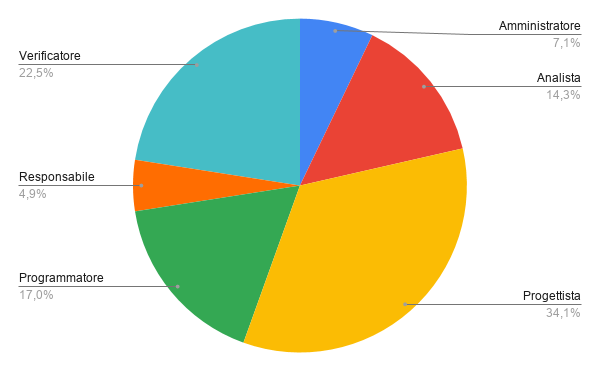
\includegraphics[width=0.8\textwidth]{source/img/architettura_ruoli.png}
        \caption{costo del personale nella fase di progettazione architetturale}
    \end{figure}
\subsection{Progettazione di dettaglio e codifica}
    \subsubsection{Prospetto orario}
    %startTable
    \def\hourlycontent{
        {Andrea Breggion,5,6,0,7,20,10,48},
        {Matteo Falsetti,5,0,0,15,15,13,48},
        {Alessandro Flori,0,4,0,10,18,16,48},
        {Andrea Mascari,0,0,0,14,22,12,48},
        {Diego Piola,5,6,0,9,20,8,48},
        {Andrea Signori,0,0,0,13,22,13,48},
        {Damiano Zanardo,0,6,0,12,20,10,48},
        {Ore totali, 15, 22, 0, 80, 137, 82, 336},
    }
    %endTable
    \newcommand*\hourlysummary{}
\foreach \x [count=\nj] in \hourlycontent
{
    \foreach \y [count=\ni] in \x
    {
        \ifnum\ni=8
            \xappto\hourlysummary{\y}
            \gappto\hourlysummary{\\}
            \gappto\hourlysummary{\hline}
        \else
            \xappto\hourlysummary{\y&}
        \fi
    }
}

% Impostazioni della tabella
\tabulinesep = 2mm % padding
\taburowcolors [1] 2{pari .. dispari} % colori delle righe
\begin{longtabu} to \textwidth {| X[0.3, c m] | X[0.1, c m] | X[0.1, c m] | X[0.1, c m] | X[0.1, c m] | X[0.1, c m] | X[0.1, c m] | X[0.1, c m] |}
\hline
\rowcolor{header} % colore dell'header
\textbf{Membro} &
\textbf{Re} & 
\textbf{Ad} & 
\textbf{An} & 
\textbf{Pt} & 
\textbf{Pr} & 
\textbf{Ve} & 
\textbf{Ore totali} \\
\hline
\hourlysummary
\end{longtabu}
\undef\hourlysummary{}
    
    \begin{figure}[H]
        \centering
        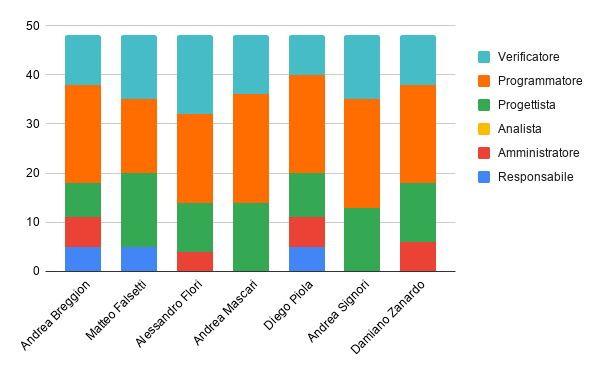
\includegraphics[width=0.8\textwidth]{source/img/codifica_orari.png}
        \caption{divisione oraria dell'attività di progettazione di dettaglio e codifica}
    \end{figure}
    \subsubsection{Prospetto economico}
    %startTable
    \def\salarycontent{
        {Amministratore,22,20,440},
        {Analista,0,25,0},
        {Progettista,80,22,1760},
        {Programmatore,137,15,2055},
        {Responsabile,15,30,450},
        {Verificatore,82,15,1230},
        {Totale,336,127,5935},
    }
    %endTable
    \newcommand*\salarysummary{}
\foreach \x [count=\nj] in \salarycontent
{
    \foreach \y [count=\ni] in \x
    {
        \ifnum\ni=1
            \xappto\salarysummary{\noexpand\textbf{\y}&}
        \else\ifnum\ni=3
            \xappto\salarysummary{\noexpand\euro\ \y&}
        \else\ifnum\ni=4
            \xappto\salarysummary{\noexpand\euro\ \y}
            \gappto\salarysummary{\\}
            \gappto\salarysummary{\hline} 
        \else
            \xappto\salarysummary{\y&}
        \fi\fi\fi
    }
}

% Impostazioni della tabella
\tabulinesep = 2mm % padding
\taburowcolors [1] 2{pari .. dispari} % colori delle righe
\begin{longtabu} to \textwidth {| X[0.1, c m] | X[0.1, c m] | X[0.1, c m] | X[0.1, c m] |}
\hline
\rowcolor{header} % colore dell'header
\textbf{Ruolo} &
\textbf{Ore} &
\textbf{Costo unitario (€)} & 
\textbf{Costo totale (€)} \\
\hline
\salarysummary
\end{longtabu}
\undef\salarysummary
    \begin{figure}[H]
        \centering
        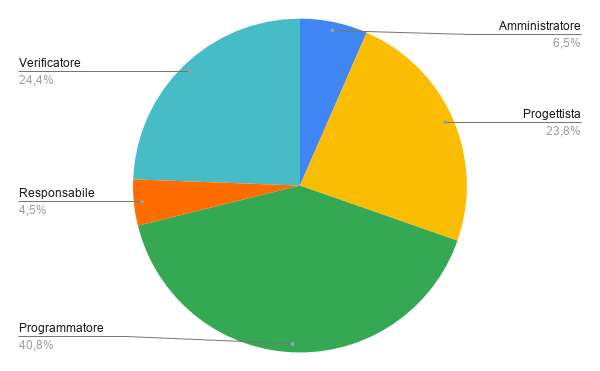
\includegraphics[width=0.8\textwidth]{source/img/codifica_ruoli.png}
        \caption{costo del personale nella fase di progettazione di dettaglio e codifica}
    \end{figure}
\subsection{Validazione e collaudo}
    \subsubsection{Prospetto orario}
    %startTable
    \def\hourlycontent{
        {Andrea Breggion,0,5,0,5,8,8,26},
        {Matteo Falsetti,0,5,0,10,5,6,26},
        {Alessandro Flori,5,0,0,7,4,10,26},
        {Andrea Mascari,0,6,0,6,5,9,26},
        {Diego Piola,0,0,0,8,8,10,26},
        {Andrea Signori,4,0,0,6,9,7,26},
        {Damiano Zanardo,6,0,0,6,4,10,26},
        {Ore totali,15,16,0,48,43,60,182},
    }
    %endTable
    \newcommand*\hourlysummary{}
\foreach \x [count=\nj] in \hourlycontent
{
    \foreach \y [count=\ni] in \x
    {
        \ifnum\ni=8
            \xappto\hourlysummary{\y}
            \gappto\hourlysummary{\\}
            \gappto\hourlysummary{\hline}
        \else
            \xappto\hourlysummary{\y&}
        \fi
    }
}

% Impostazioni della tabella
\tabulinesep = 2mm % padding
\taburowcolors [1] 2{pari .. dispari} % colori delle righe
\begin{longtabu} to \textwidth {| X[0.3, c m] | X[0.1, c m] | X[0.1, c m] | X[0.1, c m] | X[0.1, c m] | X[0.1, c m] | X[0.1, c m] | X[0.1, c m] |}
\hline
\rowcolor{header} % colore dell'header
\textbf{Membro} &
\textbf{Re} & 
\textbf{Ad} & 
\textbf{An} & 
\textbf{Pt} & 
\textbf{Pr} & 
\textbf{Ve} & 
\textbf{Ore totali} \\
\hline
\hourlysummary
\end{longtabu}
\undef\hourlysummary{}
    \begin{figure}[H]
        \centering
        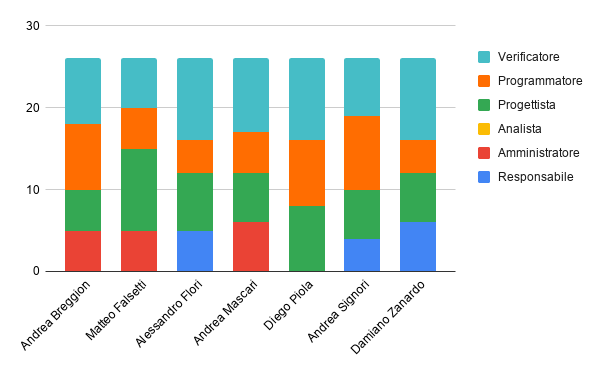
\includegraphics[width=0.8\textwidth]{source/img/validazione_orari.png}
        \caption{divisione oraria dell'attività di validazione e collaudo}
    \end{figure}
    \subsubsection{Prospetto economico}
    %startTable
    \def\salarycontent{
        {Amministratore,16,20,320},
        {Analista,0,25,0},
        {Progettista,48,22,1056},
        {Programmatore,43,15,645},
        {Responsabile,15,30,450},
        {Verificatore,60,15,900},
        {Totale,182,127,3371},
    }
    %endTable
    \newcommand*\salarysummary{}
\foreach \x [count=\nj] in \salarycontent
{
    \foreach \y [count=\ni] in \x
    {
        \ifnum\ni=1
            \xappto\salarysummary{\noexpand\textbf{\y}&}
        \else\ifnum\ni=3
            \xappto\salarysummary{\noexpand\euro\ \y&}
        \else\ifnum\ni=4
            \xappto\salarysummary{\noexpand\euro\ \y}
            \gappto\salarysummary{\\}
            \gappto\salarysummary{\hline} 
        \else
            \xappto\salarysummary{\y&}
        \fi\fi\fi
    }
}

% Impostazioni della tabella
\tabulinesep = 2mm % padding
\taburowcolors [1] 2{pari .. dispari} % colori delle righe
\begin{longtabu} to \textwidth {| X[0.1, c m] | X[0.1, c m] | X[0.1, c m] | X[0.1, c m] |}
\hline
\rowcolor{header} % colore dell'header
\textbf{Ruolo} &
\textbf{Ore} &
\textbf{Costo unitario (€)} & 
\textbf{Costo totale (€)} \\
\hline
\salarysummary
\end{longtabu}
\undef\salarysummary
    \label{image:verifica_ruoli}
    \begin{figure}[H]
        \centering
        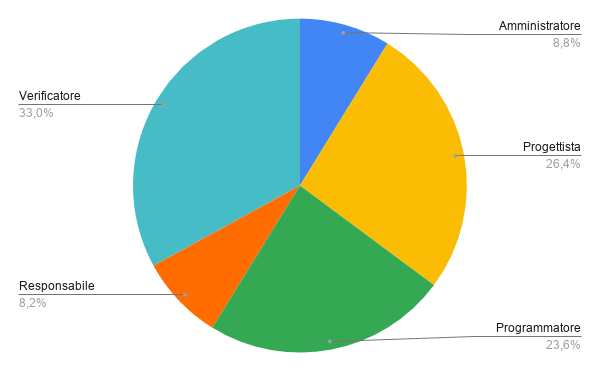
\includegraphics[width=0.8\textwidth]{source/img/validazione_ruoli.png}
        \caption{costo del personale nella fase di validazione e collaudo}
    \end{figure}
\subsection{Riepilogo}
    \subsection{Ore totali}
    All'interno di questa sottosezione è contenuto il riepilogo delle ore totali, comprensive dell'investimento, che non sarà rendicontato nell'offerta finale, ossia della fase di analisi.
        \paragraph{Suddivisione del lavoro}
        
        %startTable
        \def\hourlycontent{
            {Andrea Breggion,11,35,7,18,33,30,134},
            {Matteo Falsetti,5,10,8,43,20,48,134},
            {Alessandro Flori,7,8,10,36,22,51,134},
            {Andrea Mascari,4,6,19,33,33,39,134},
            {Diego Piola,18,19,12,26,34,25,134},
            {Andrea Signori,16,12,10,26,36,34,134},
            {Damiano Zanardo,6,13,19,30,33,33,134},
            {Ore totali,67,103,85,212,211,260,938},
        }
        %endTable
        \newcommand*\hourlysummary{}
\foreach \x [count=\nj] in \hourlycontent
{
    \foreach \y [count=\ni] in \x
    {
        \ifnum\ni=8
            \xappto\hourlysummary{\y}
            \gappto\hourlysummary{\\}
            \gappto\hourlysummary{\hline}
        \else
            \xappto\hourlysummary{\y&}
        \fi
    }
}

% Impostazioni della tabella
\tabulinesep = 2mm % padding
\taburowcolors [1] 2{pari .. dispari} % colori delle righe
\begin{longtabu} to \textwidth {| X[0.3, c m] | X[0.1, c m] | X[0.1, c m] | X[0.1, c m] | X[0.1, c m] | X[0.1, c m] | X[0.1, c m] | X[0.1, c m] |}
\hline
\rowcolor{header} % colore dell'header
\textbf{Membro} &
\textbf{Re} & 
\textbf{Ad} & 
\textbf{An} & 
\textbf{Pt} & 
\textbf{Pr} & 
\textbf{Ve} & 
\textbf{Ore totali} \\
\hline
\hourlysummary
\end{longtabu}
\undef\hourlysummary{} 
        \begin{figure}[H]
            \centering
            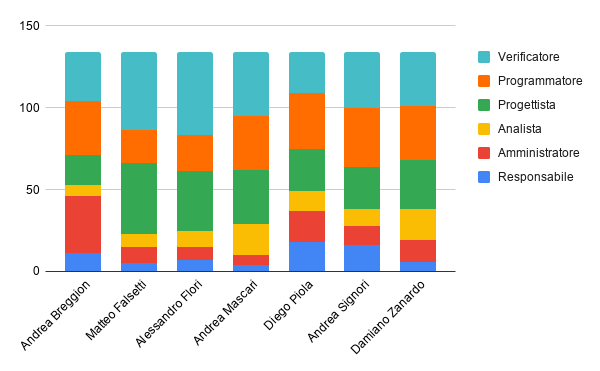
\includegraphics[width=0.8\textwidth]{source/img/totale_orari.png}
            \caption{divisione oraria complessiva}
        \end{figure}
        \paragraph{Prospetto economico}
        
        %startTable
        \def\salarycontent{
            {Amministratore,103,20,2060},
            {Analista,85,25,2125},
            {Progettista,212,22,4664},
            {Programmatore,211,15,3165},
            {Responsabile,67,30,2010},
            {Verificatore,260,15,3900},
            {Totale,938,127,17924},
        }
        %endTable
        \newcommand*\salarysummary{}
\foreach \x [count=\nj] in \salarycontent
{
    \foreach \y [count=\ni] in \x
    {
        \ifnum\ni=1
            \xappto\salarysummary{\noexpand\textbf{\y}&}
        \else\ifnum\ni=3
            \xappto\salarysummary{\noexpand\euro\ \y&}
        \else\ifnum\ni=4
            \xappto\salarysummary{\noexpand\euro\ \y}
            \gappto\salarysummary{\\}
            \gappto\salarysummary{\hline} 
        \else
            \xappto\salarysummary{\y&}
        \fi\fi\fi
    }
}

% Impostazioni della tabella
\tabulinesep = 2mm % padding
\taburowcolors [1] 2{pari .. dispari} % colori delle righe
\begin{longtabu} to \textwidth {| X[0.1, c m] | X[0.1, c m] | X[0.1, c m] | X[0.1, c m] |}
\hline
\rowcolor{header} % colore dell'header
\textbf{Ruolo} &
\textbf{Ore} &
\textbf{Costo unitario (€)} & 
\textbf{Costo totale (€)} \\
\hline
\salarysummary
\end{longtabu}
\undef\salarysummary
        \begin{figure}[H]
            \centering
            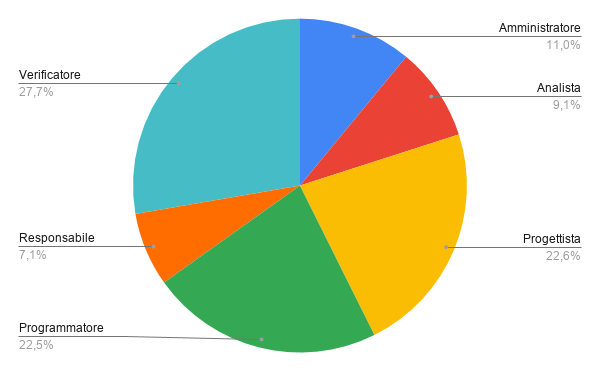
\includegraphics[width=0.8\textwidth]{source/img/totale_ruoli.png}
            \caption{costo del personale complessivo}
        \end{figure}
    \subsection{Ore rendicontate}
    All'interno di questa sottosezione è contenuto il riepilogo delle ore dedicate all'attività di progetto nonché il riepilogo dei costi relativi al periodo successivo alla RR.
        \paragraph{Suddivisione del lavoro}
        
        %startTable
        \def\hourlycontent{
            {Andrea Breggion,5,21,4,18,33,24,105},
            {Matteo Falsetti,5,5,5,33,20,37,105},
            {Alessandro Flori,5,4,7,28,22,39,105},
            {Andrea Mascari,4,6,5,31,33,26,105},
            {Diego Piola,12,6,9,26,34,18,105},
            {Andrea Signori,4,6,6,26,36,27,105},
            {Damiano Zanardo,6,6,5,30,33,25,105},
            {Ore totali,41,54,41,192,211,196,735},
        }
        %endTable
        \newcommand*\hourlysummary{}
\foreach \x [count=\nj] in \hourlycontent
{
    \foreach \y [count=\ni] in \x
    {
        \ifnum\ni=8
            \xappto\hourlysummary{\y}
            \gappto\hourlysummary{\\}
            \gappto\hourlysummary{\hline}
        \else
            \xappto\hourlysummary{\y&}
        \fi
    }
}

% Impostazioni della tabella
\tabulinesep = 2mm % padding
\taburowcolors [1] 2{pari .. dispari} % colori delle righe
\begin{longtabu} to \textwidth {| X[0.3, c m] | X[0.1, c m] | X[0.1, c m] | X[0.1, c m] | X[0.1, c m] | X[0.1, c m] | X[0.1, c m] | X[0.1, c m] |}
\hline
\rowcolor{header} % colore dell'header
\textbf{Membro} &
\textbf{Re} & 
\textbf{Ad} & 
\textbf{An} & 
\textbf{Pt} & 
\textbf{Pr} & 
\textbf{Ve} & 
\textbf{Ore totali} \\
\hline
\hourlysummary
\end{longtabu}
\undef\hourlysummary{}
        \begin{figure}[H]
            \centering
            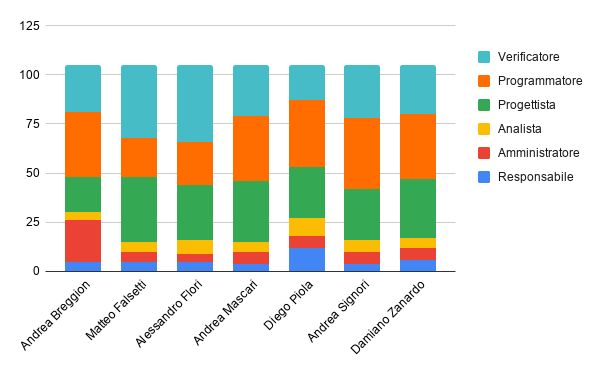
\includegraphics[width=0.8\textwidth]{source/img/no_investimento_orari.png}
            \caption{divisione oraria totale senza l'investimento iniziale}
        \end{figure}
        \paragraph{Prospetto economico}
        
        %startTable
        \def\salarycontent{
            {Amministratore,54,20,1080},
            {Analista,41,25,1025},
            {Progettista,192,22,4224},
            {Programmatore,211,15,3165},
            {Responsabile,41,30,1230},
            {Verificatore,196,15,2940},
            {Totale,735,127,13664},
        }
        %endTable
        \newcommand*\salarysummary{}
\foreach \x [count=\nj] in \salarycontent
{
    \foreach \y [count=\ni] in \x
    {
        \ifnum\ni=1
            \xappto\salarysummary{\noexpand\textbf{\y}&}
        \else\ifnum\ni=3
            \xappto\salarysummary{\noexpand\euro\ \y&}
        \else\ifnum\ni=4
            \xappto\salarysummary{\noexpand\euro\ \y}
            \gappto\salarysummary{\\}
            \gappto\salarysummary{\hline} 
        \else
            \xappto\salarysummary{\y&}
        \fi\fi\fi
    }
}

% Impostazioni della tabella
\tabulinesep = 2mm % padding
\taburowcolors [1] 2{pari .. dispari} % colori delle righe
\begin{longtabu} to \textwidth {| X[0.1, c m] | X[0.1, c m] | X[0.1, c m] | X[0.1, c m] |}
\hline
\rowcolor{header} % colore dell'header
\textbf{Ruolo} &
\textbf{Ore} &
\textbf{Costo unitario (€)} & 
\textbf{Costo totale (€)} \\
\hline
\salarysummary
\end{longtabu}
\undef\salarysummary
        \begin{figure}[H]
            \centering
            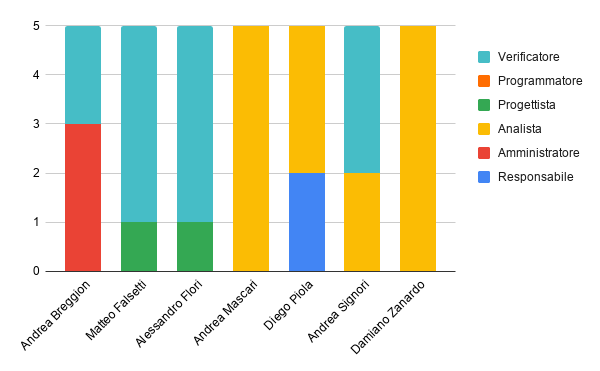
\includegraphics[width=0.8\textwidth]{source/img/consolidamento_orari.png}
            \caption{costo totale del personale senza l'investimento iniziale}
        \end{figure}
    \subsection{Conclusioni}
    All'interno della tabella di cui sopra è indicata l'offerta con cui Code of Duty si presenta al committente. Tale somma ammonta a \euro\ 13664.

    \pagebreak
    \section{Analisi degli scostamenti} 

\subsection{Consuntivo del periodo di analisi}

Durante il periodo di analisi sono state rilevate più ore rispetto a quanto preventivato per i ruoli di:

\begin{itemize}
    \item \textbf{Amministratore:} è stato dedicato più tempo del previsto per impostare l'ambiente di sviluppo, in modo da automatizzare il più possibile i processi di rilascio della documentazione, nonché la raccolta delle metriche;
    \item \textbf{Verificatore:} essendo questa la prima fase del progetto, il team ha deciso di investire più ore rispetto a quanto preventivato nell'attività di verifica allo scopo di preparare dei documenti il più completi e coerenti possibile.
\end{itemize}

%startTable
\def\salarycontent{
    {Amministratore,$49+\noexpand\textbf{15}=64$,20,1280},
    {Analista,44,25,1100},
    {Progettista,20,22,440},
    {Programmatore,0,15,0},
    {Responsabile,26,30,780},
    {Verificatore,$64+\noexpand\textbf{10}=74$,15,1110},
    {Totale,203,127,4710},
}
%endTable
\newcommand*\salarysummary{}
\foreach \x [count=\nj] in \salarycontent
{
    \foreach \y [count=\ni] in \x
    {
        \ifnum\ni=1
            \xappto\salarysummary{\noexpand\textbf{\y}&}
        \else\ifnum\ni=3
            \xappto\salarysummary{\noexpand\euro\ \y&}
        \else\ifnum\ni=4
            \xappto\salarysummary{\noexpand\euro\ \y}
            \gappto\salarysummary{\\}
            \gappto\salarysummary{\hline} 
        \else
            \xappto\salarysummary{\y&}
        \fi\fi\fi
    }
}

% Impostazioni della tabella
\tabulinesep = 2mm % padding
\taburowcolors [1] 2{pari .. dispari} % colori delle righe
\begin{longtabu} to \textwidth {| X[0.1, c m] | X[0.1, c m] | X[0.1, c m] | X[0.1, c m] |}
\hline
\rowcolor{header} % colore dell'header
\textbf{Ruolo} &
\textbf{Ore} &
\textbf{Costo unitario (€)} & 
\textbf{Costo totale (€)} \\
\hline
\salarysummary
\end{longtabu}
\undef\salarysummary
\noindent Gli scostamenti rilevati hanno quindi causato un aumento dell'investimento di $4710 - 4260 =$ \euro\ 450.
Per completezza viene mostrato il preventivo a finire tenendo conto del periodo di investimento, si noti che non indica una modifica dell'offerta.
%startTable
\def\salarycontent{
    {Amministratore,$103+\noexpand\textbf{15}$,20,2360},
    {Analista,85,25,2125},
    {Progettista,212,22,4664},
    {Programmatore,211,15,3165},
    {Responsabile,67,30,2010},
    {Verificatore,$260+\noexpand\textbf{10}$,15,4050},
    {Totale,938,127,18374},
}
%endTable
\newcommand*\salarysummary{}
\foreach \x [count=\nj] in \salarycontent
{
    \foreach \y [count=\ni] in \x
    {
        \ifnum\ni=1
            \xappto\salarysummary{\noexpand\textbf{\y}&}
        \else\ifnum\ni=3
            \xappto\salarysummary{\noexpand\euro\ \y&}
        \else\ifnum\ni=4
            \xappto\salarysummary{\noexpand\euro\ \y}
            \gappto\salarysummary{\\}
            \gappto\salarysummary{\hline} 
        \else
            \xappto\salarysummary{\y&}
        \fi\fi\fi
    }
}

% Impostazioni della tabella
\tabulinesep = 2mm % padding
\taburowcolors [1] 2{pari .. dispari} % colori delle righe
\begin{longtabu} to \textwidth {| X[0.1, c m] | X[0.1, c m] | X[0.1, c m] | X[0.1, c m] |}
\hline
\rowcolor{header} % colore dell'header
\textbf{Ruolo} &
\textbf{Ore} &
\textbf{Costo unitario (€)} & 
\textbf{Costo totale (€)} \\
\hline
\salarysummary
\end{longtabu}
\undef\salarysummary
\noindent Con una differenza rispetto a quanto preventivato di \euro\ 450.
\subsubsection{Preventivo a finire}
Il preventivo e quindi l'offerta rimangono invariati rispetto a quanto è stato presentato nella sezione dedicata. Le ore aggiuntive rilevate per quanto riguarda i ruoli di Amministratore e Verificatore sono considerate (esattamente come l'intero periodo di Analisi) un investimento e non sono causa di aggiustamenti in aumento: 
\begin{itemize}
    \item \textbf{Amministratore:} l'aver speso più ore del previsto per impostare l'ambiente di lavoro sarà sicuramente un vantaggio nelle fasi successive del progetto;
    \item \textbf{Verificatore:} ora che i documenti sono stati avviati, si stima che l'attività di verifica rientrerà nei limiti previsti.
\end{itemize}

\subsection{Consuntivo del periodo di consolidamento dei requisiti}
Durante questa fase non si sono verificati scostamenti per quanto riguarda le ore preventivate. 

\subsection{Consuntivo del periodo di progettazione architetturale}
Durante il periodo di progettazione architetturale il team ha realizzato un Proof of Concept che dimostrasse la fattibilità di \hd\ con le tecnologie individuate (VI021), questo ha richiesto un grande impegno per quanto riguarda l'autoformazione, impegno purtroppo non contabilizzabile. 
Si riporta quanto segue:
\begin{itemize}
    \item \textbf{Analista}: le segnalazioni riportate in fase della correzione della RR hanno richiesto maggior impegno da parte degli analisti;
    \item \textbf{Programmatore e Progettista}: una volta scelte le tecnologie l'integrazione di queste ha richiesto più lavoro rispetto a quanto preventivato, è stato quindi scelto di dedicare più ore alla programmazione a discapito della progettazione.
\end{itemize}
%startTable
\def\salarycontent{
    {Amministratore,13,20,260},
    {Analista,$26+\noexpand\textbf{6}$,25,800},
    {Progettista,$62-\noexpand\textbf{10}$,22,1144},
    {Programmatore,$31+\noexpand\textbf{10}$,15,615},
    {Responsabile,9,30,270},
    {Verificatore,41,15,615},
    {Totale,188,127,3704},
}
%endTable
\newcommand*\salarysummary{}
\foreach \x [count=\nj] in \salarycontent
{
    \foreach \y [count=\ni] in \x
    {
        \ifnum\ni=1
            \xappto\salarysummary{\noexpand\textbf{\y}&}
        \else\ifnum\ni=3
            \xappto\salarysummary{\noexpand\euro\ \y&}
        \else\ifnum\ni=4
            \xappto\salarysummary{\noexpand\euro\ \y}
            \gappto\salarysummary{\\}
            \gappto\salarysummary{\hline} 
        \else
            \xappto\salarysummary{\y&}
        \fi\fi\fi
    }
}

% Impostazioni della tabella
\tabulinesep = 2mm % padding
\taburowcolors [1] 2{pari .. dispari} % colori delle righe
\begin{longtabu} to \textwidth {| X[0.1, c m] | X[0.1, c m] | X[0.1, c m] | X[0.1, c m] |}
\hline
\rowcolor{header} % colore dell'header
\textbf{Ruolo} &
\textbf{Ore} &
\textbf{Costo unitario (€)} & 
\textbf{Costo totale (€)} \\
\hline
\salarysummary
\end{longtabu}
\undef\salarysummary
\noindent Gli scostamenti rilevati hanno quindi causato un aumento del costo del periodo di $3704 - 3624 =$ \euro\ 80.

\subsubsection{Preventivo a finire}
L'aver dedicato più tempo alla programmazione a discapito della progettazione ha le seguenti conseguenze:
\begin{itemize}
    \item potrebbe essere causa di refactoring che aumenterebbe il carico di lavoro dei programmatori;
    \item i programmatori hanno confidenza con le tecnologie adottate.
\end{itemize}
È stato deciso di modificare il prospetto orario della fase successiva (Progettazione di dettaglio e codifica) ridistribuendo le ore tra programmatori e progettisti allo scopo di evitare i problemi sopra citati e ridurre l'aumento dell'offerta causato dallo scostamento riportato.

\label{table:nuovo_orario_codifica}
%startTable
\def\salarycontent{
    {Amministratore,22,20,440},
    {Analista,0,25,0},
    {Progettista,$80+\noexpand\textbf{10}$,22,1980},
    {Programmatore,$137-\noexpand\textbf{17}$,15,1800},
    {Responsabile,15,30,450},
    {Verificatore,82,15,1230},
    {Totale,329,127,$5935-\noexpand\textbf{35} = 5900 $ },
}
%endTable
\newcommand*\salarysummary{}
\foreach \x [count=\nj] in \salarycontent
{
    \foreach \y [count=\ni] in \x
    {
        \ifnum\ni=1
            \xappto\salarysummary{\noexpand\textbf{\y}&}
        \else\ifnum\ni=3
            \xappto\salarysummary{\noexpand\euro\ \y&}
        \else\ifnum\ni=4
            \xappto\salarysummary{\noexpand\euro\ \y}
            \gappto\salarysummary{\\}
            \gappto\salarysummary{\hline} 
        \else
            \xappto\salarysummary{\y&}
        \fi\fi\fi
    }
}

% Impostazioni della tabella
\tabulinesep = 2mm % padding
\taburowcolors [1] 2{pari .. dispari} % colori delle righe
\begin{longtabu} to \textwidth {| X[0.1, c m] | X[0.1, c m] | X[0.1, c m] | X[0.1, c m] |}
\hline
\rowcolor{header} % colore dell'header
\textbf{Ruolo} &
\textbf{Ore} &
\textbf{Costo unitario (€)} & 
\textbf{Costo totale (€)} \\
\hline
\salarysummary
\end{longtabu}
\undef\salarysummary

\noindent I costi rilevati ammontano quindi a: \euro\ 13704. \cod\ si impegna a riportare i costi a quanto preventivato in sede di RA.

\subsection{Consuntivo del periodo di progettazione di dettaglio e codifica}
Durante questa fase il team ha portato a termine la Product Baseline, arrivando ad una architettura definitiva.
In particolare sono già stati implementati la maggior parte dei requisiti funzionali indicati nel documento \AdR .
Nonostante il verificarsi dei rischi \hyperref[section:rischi_rilevati]{RO3-0}, \hyperref[section:rischi_rilevati]{RO2-1},
è stato rispettato il preventivo orario deciso nel periodo precedente. 
Per semplicità è fornito un riferimento al prospetto economico sopra citato: \hyperref[table:nuovo_orario_codifica]{link}.
    \subsubsection{Preventivo a finire}
        A seguito del periodo, si riporta comunque una differenza in aumento rispetto all'offerta finale di \euro\ 45,
        tale differenza \textbf{non} porta ad una effettiva modifica dell'offerta finale, tuttavia è segno di una pianificazione non precisa,
        oltre che di uno spreco di risorse.
        Il team si impegna entro il termine della prossima e ultima fase a riportare i costi entro l'offerta fissata e a tal proposito propone
        un nuovo prospetto orario per la fase successiva di validazione e collaudo.
        %startTable
        \def\salarycontent{
            {Amministratore,16,20,320},
            {Analista,0,25,0},
            {Progettista,$48-\noexpand\textbf{8}$,22,880},
            {Programmatore,$43+\noexpand\textbf{7}$,15,750},
            {Responsabile,15,30,450},
            {Verificatore,60,15,900},
            {Totale,181,127,$3371-\noexpand\textbf{71} = 3300 $ },
        }
        %endTable
        \newcommand*\salarysummary{}
\foreach \x [count=\nj] in \salarycontent
{
    \foreach \y [count=\ni] in \x
    {
        \ifnum\ni=1
            \xappto\salarysummary{\noexpand\textbf{\y}&}
        \else\ifnum\ni=3
            \xappto\salarysummary{\noexpand\euro\ \y&}
        \else\ifnum\ni=4
            \xappto\salarysummary{\noexpand\euro\ \y}
            \gappto\salarysummary{\\}
            \gappto\salarysummary{\hline} 
        \else
            \xappto\salarysummary{\y&}
        \fi\fi\fi
    }
}

% Impostazioni della tabella
\tabulinesep = 2mm % padding
\taburowcolors [1] 2{pari .. dispari} % colori delle righe
\begin{longtabu} to \textwidth {| X[0.1, c m] | X[0.1, c m] | X[0.1, c m] | X[0.1, c m] |}
\hline
\rowcolor{header} % colore dell'header
\textbf{Ruolo} &
\textbf{Ore} &
\textbf{Costo unitario (€)} & 
\textbf{Costo totale (€)} \\
\hline
\salarysummary
\end{longtabu}
\undef\salarysummary
        \label{table:nuovo_orario_verifica}
        Si può notare una diminuzione delle ore del ruolo di progettista, possibile grazie
        al buon lavoro svolto durante la fase di progettazione di dettaglio e codifica.
        Inoltre sono state assegnate più ore al programmatore in quanto sono ancora da definire
        i test di unità e integrazione, nonché alcuni requisiti da implementare. \\
        \noindent Queste modifiche portano l'offerta finale al nuovo valore di \euro\ 13638 contro
        i \euro\ 13664 preventivati.

    \pagebreak
    \appendix
    \section{Attualizzazione dei rischi}
\label{section:rischi_rilevati}
In questo appendice sono raccolti i problemi verificati durante l'attività di progetto ed è riportata la soluzione attuata o la situazione del problema al momento della redazione di questo documento.
Ogni rischio rilevato ha associato un codice: \\
\textit{identificativoRischio-numeroIncrementale} e.g. RT1-0. \\
\noindent Un rischio può essere:
\begin{itemize}
    \item non superato;
    \item parzialmente superato;
    \item superato.
\end{itemize}
\subsection{Rischi tecnologici verificati}
%startTable
\def\problems{
    {   
        RT1-0,
        \noexpand\textbf{Fase rilevazione:} progettazione architetturale \noexpand\newline
        Alcuni membri del gruppo non conoscono o non sono pratici dello strumento Github.,
        Tali membri hanno dedicato allo strumento un breve periodo di autoformazione prima d'iniziare l'esperienza sul campo. I membri più esperti del team sono stati e resteranno sempre disponibili per chiarimenti.,
        \noexpand\textbf{Ultimo aggiornamento:} 2021-04-03 \noexpand\newline
        Il rischio risulta superato.
    },
    {
        RT1-1,
        \noexpand\textbf{Fase rilevazione:} analisi \noexpand\newline
        L'esperienza con LaTeX da parte del team (nella sua interezza) è poca o nulla.,
        La redazione dei documenti si è inizialmente rivelato un processo lento e frustrante{,} tuttavia è stato considerato un male necessario. Ancora adesso si riscontrano difficoltà rispetto alla creazione di tabelle e posizionamento di immagini.,
        \noexpand\textbf{Ultimo aggiornamento:} 2021-04-03 \noexpand\newline
        Il rischio risulta superato.
    },
    {   
        RT1-2,
        \noexpand\textbf{Fase rilevazione:} progettazione architetturale \noexpand\newline
        Nessun membro del gruppo è pratico o ha conoscenze approfondite delle tecnologie coinvolte per la realizzazione del POC.,
        È stato dedicato un periodo di 2 settimane all'autoapprendimento delle tecnologie coinvolte{,} in particolare è stato deciso che ogni membro del gruppo deve avere per ognuna una conoscenza almeno superficiale.,
        \noexpand\textbf{Ultimo aggiornamento:} 2021-04-03 \noexpand\newline
        Ogni membro del gruppo è specializzato in una particolare tecnologia{,} tuttavia queste non sono ancora completamente padroneggiate. Sebbene contenuto il rischio risulta parzialmente superato.
    },
}
%endTable
\newcommand*\improvementeval{}
\foreach \x [count=\nj] in \problems
{
    \foreach \y [count=\ni] in \x
    {
        \ifnum\ni=1
            \xappto\improvementeval{\noexpand\textbf{\y}&}
        \else\ifnum\ni=4
            \xappto\improvementeval{\y}
            \gappto\improvementeval{\\}
            \gappto\improvementeval{\hline}
        \else
            \xappto\improvementeval{\y&}
        \fi\fi
    }
}

% Impostazioni della tabella
\tabulinesep = 2mm % padding
\taburowcolors [1] 2{pari .. dispari} % colori delle righe
\begin{longtabu} to \textwidth {| X[0.1,c m] | X[0.2,c m] | X[0.3,l m] | X[0.3,l m] |} % larghezza delle colonne
\hline
\rowcolor{header} % colore dell'header

\textbf{Codice rischio} & \textbf{Problema} & \textbf{Descrizione} & \textbf{Soluzione} \\
\hline
\improvementeval

\end{longtabu}

\undef\improvementeval{}

\subsection{Rischi organizzativi verificati}
%startTable
\def\problems{
    {
        RO1-0,
        \noexpand\textbf{Fase rilevazione:} analisi \noexpand\newline
        Risulta complicato trovare un giorno e anche un orario per svolgere gli incontri.,
        Grazie al supporto dei canali di comunicazione individuati dalle \noexpand\NdP\ e all'attività di verbalizzazione non è necessario che sia presente l'intero team ogni incontro. Per gli incontri più importanti{,} dove è necessario che sia presente tutto il gruppo{,} è necessario mettersi d'accordo con largo anticipo.,
        \noexpand\textbf{Ultimo aggiornamento:} 2021-04-03 \noexpand\newline
        Il team è più affiatato{,} gli incontri sono molto più frequenti anche se si sono trasformati in lavoro collaborativo{,} la maggior parte delle decisioni viene presa in modalità asincrona. Il rischio risulta superato.
    },
    {
        RO1-1,
        \noexpand\textbf{Fase rilevazione:} analisi \noexpand\newline
        Il ruolo di amministratore ha richiesto più ore rispetto a quanto preventivato{,} come riportato nel \noexpand\PdP {,} è stato dedicato molto tempo a impostare la repository e le GitHub Actions{,} con l'obiettivo di automatizzare il più possibile alcune operazioni.,
        Non sono state considerate azioni di mitigazione.,
        \noexpand\textbf{Ultimo aggiornamento:} 2021-04-03 \noexpand\newline
        L'aver dedicato molte ore nell'impostare l'ambiente di sviluppo è sicuramente un investimento per il futuro{,} sia per quanto riguarda il prodotto del processo di documentazione che per il prodotto software{,} infatti impostare la repository dedicata al codice sarà sicuramente un processo più agevole. Il rischio risulta superato.
    },
    {
        RO1-2,
        \noexpand\textbf{Fase rilevazione:} progettazione architetturale \noexpand\newline
        Causato da RT1-2{,} i programmatori hanno avuto bisogno di più tempo di quanto preventivato per utilizzare efficacemente le tecnologie richieste per la realizzazione del POC.,
        È stato tolto del tempo alla progettazione per concentrarsi maggiormente alla programmazione.,
        \noexpand\textbf{Ultimo aggiornamento:} 2021-04-03 \noexpand\newline
        Il rischio è stato superato.
    },
    {
        RO2-0,
        \noexpand\textbf{Fase rilevazione:} progettazione architetturale \noexpand\newline
        La sessione invernale è stata particolarmente impegnativa per la maggior parte del gruppo.,
        È stata utilizzata la revisione a modalità \noexpand\textit{Sportello}: il team ha deciso di ritardare la consegna della Technology Baseline{,} nonché la consegna dei documenti per la RP rispettivamente al 2021-03-09 e al 2021-03-10.,
        \noexpand\textbf{Ultimo aggiornamento:} 2021-04-03 \noexpand\newline
        Il rischio è stato superato.
    },
    {
        RO2-1,
        \noexpand\textbf{Fase rilevazione:} progettazione architetturale \noexpand\newline
        Tre membri del team hanno deciso di sostenere l'esame teorico di Ingegneria del Software{,} ha richiesto un periodo di preparazione 
        (una settimana circa).,
        Il lavoro assegnato ai membri temporaneamente poco produttivi è stato ridistribuito,
        \noexpand\textbf{Ultimo aggiornamento:} 2021-04-18 \noexpand\newline
        Il rischio è stato superato{,} inoltre lo slittamento dell'inizio dei colloqui per l'approvazione della Product Baseline 
        ha permesso un certo \noexpand\textit{slack}.
    },
    {
        RO3-0,
        \noexpand\textbf{Fase rilevazione:} progettazione di dettaglio e codifica \noexpand\newline
        Un membro del team si è rimasto assente per  una settimana.,
        Non sono state effettuate azioni di mitigazione: le attività in gestione al membro erano buono stato di avanzamento,
        \noexpand\textbf{Ultimo aggiornamento:} 2021-04-18 \noexpand\newline
        Il rischio è stato superato{,} inoltre lo slittamento dell'inizio dei colloqui per l'approvazione della Product Baseline 
        ha permesso un certo \noexpand\textit{slack}.
    },
}
%endTable

% RO2-1 3 membri del team operatività ridotta per preparazione scritto di SWE
\newcommand*\improvementeval{}
\foreach \x [count=\nj] in \problems
{
    \foreach \y [count=\ni] in \x
    {
        \ifnum\ni=1
            \xappto\improvementeval{\noexpand\textbf{\y}&}
        \else\ifnum\ni=4
            \xappto\improvementeval{\y}
            \gappto\improvementeval{\\}
            \gappto\improvementeval{\hline}
        \else
            \xappto\improvementeval{\y&}
        \fi\fi
    }
}

% Impostazioni della tabella
\tabulinesep = 2mm % padding
\taburowcolors [1] 2{pari .. dispari} % colori delle righe
\begin{longtabu} to \textwidth {| X[0.1,c m] | X[0.2,c m] | X[0.3,l m] | X[0.3,l m] |} % larghezza delle colonne
\hline
\rowcolor{header} % colore dell'header

\textbf{Codice rischio} & \textbf{Problema} & \textbf{Descrizione} & \textbf{Soluzione} \\
\hline
\improvementeval

\end{longtabu}

\undef\improvementeval{}

\subsection{Riepilogo rischi verificati}
    %startTable
    \tabulinesep = 2mm % padding
    \taburowcolors [1] 2{pari .. dispari} % colori delle righe
    \begin{longtabu} to \textwidth {| X[0.1,c m] | X[0.1,c m] |} % larghezza delle colonne
        \hline
        \rowcolor{header} % colore dell'header

        \textbf{Rischio verificato} & \textbf{Status} \\
        \hline

        \textbf{RT1-0} & superato\\
        \hline 
        \textbf{RT1-1} & superato\\
        \hline
        \textbf{RT1-2} & parzialmente superato\\
        \hline
        \textbf{RO1-0} & superato \\ 
        \hline
        \textbf{RO1-1} & superato \\ 
        \hline
        \textbf{RO1-2} & superato \\ 
        \hline
        \textbf{RO2-0} & superato \\ 
        \hline

    \end{longtabu}
    %endTable

    \pagebreak
    \section{Organigramma}
\subsection{Redazione}
%startTable
\def\staff{
    {
        \noexpand\textbf{Nominativo},
        \noexpand\textbf{Data redazione},
        \noexpand\textbf{Firma}
    },
    {
        Alessandro Flori,
        2020-01-10,
        -
    },
    {
        Andrea Signori,
        2020-01-10,
        -
    },
}
%endTable
\newcommand*\organigramma{}
\foreach \x [count=\nj] in \staff
{
    \foreach \y [count=\ni] in \x
    {
        \ifnum\ni=3
            \xappto\organigramma{\y}
            \gappto\organigramma{\\}
            \gappto\organigramma{\hline}
        \else
            \xappto\organigramma{\y&}
        \fi
    }
}

% Impostazioni della tabella
\tabulinesep = 2mm % padding
\taburowcolors [1] 2{pari .. dispari} % colori delle righe
\begin{longtabu} to \textwidth {| X[0.2,c m] | X[0.1,c m] | X[0.3,c m] |} % larghezza delle colonne
\hline
\rowcolor{header} % colore dell'header
\organigramma

\end{longtabu}

\undef\organigramma{}


\subsection{Approvazione}
%startTable
\def\staff{
    {
        \noexpand\textbf{Nominativo},
        \noexpand\textbf{Data approvazione},
        \noexpand\textbf{Firma}
    },
    {
        Andrea Breggion,
        2020-01-11,
        -
    },
}
%endTable
\newcommand*\organigramma{}
\foreach \x [count=\nj] in \staff
{
    \foreach \y [count=\ni] in \x
    {
        \ifnum\ni=3
            \xappto\organigramma{\y}
            \gappto\organigramma{\\}
            \gappto\organigramma{\hline}
        \else
            \xappto\organigramma{\y&}
        \fi
    }
}

% Impostazioni della tabella
\tabulinesep = 2mm % padding
\taburowcolors [1] 2{pari .. dispari} % colori delle righe
\begin{longtabu} to \textwidth {| X[0.2,c m] | X[0.1,c m] | X[0.3,c m] |} % larghezza delle colonne
\hline
\rowcolor{header} % colore dell'header
\organigramma

\end{longtabu}

\undef\organigramma{}


\subsection{Accettazione dei componenti}
%startTable
\def\staff{
    {
        \noexpand\textbf{Nominativo},
        \noexpand\textbf{Data accettazione},
        \noexpand\textbf{Firma}
    },
    {
        Andrea Breggion,
        2020-01-10,
        -
    },
    {
        Matteo Falsetti,
        2020-01-10,
        -
    },
    {
        Alessandro Flori,
        2020-01-10,
        -
    },
    {
        Andrea Mascari,
        2020-01-10,
        -
    },
    {
        Diego Piola,
        2020-01-10,
        -
    },
    {
        Andrea Signori,
        2020-01-10,
        -
    },
    {
        Damiano Zanardo,
        2020-01-10,
        -
    },
}
%endTable
\newcommand*\organigramma{}
\foreach \x [count=\nj] in \staff
{
    \foreach \y [count=\ni] in \x
    {
        \ifnum\ni=3
            \xappto\organigramma{\y}
            \gappto\organigramma{\\}
            \gappto\organigramma{\hline}
        \else
            \xappto\organigramma{\y&}
        \fi
    }
}

% Impostazioni della tabella
\tabulinesep = 2mm % padding
\taburowcolors [1] 2{pari .. dispari} % colori delle righe
\begin{longtabu} to \textwidth {| X[0.2,c m] | X[0.1,c m] | X[0.3,c m] |} % larghezza delle colonne
\hline
\rowcolor{header} % colore dell'header
\organigramma

\end{longtabu}

\undef\organigramma{}


\subsection{Componenti}
%startTable
\def\staff{
    {
        \noexpand\textbf{Nominativo},
        \noexpand\textbf{Matricola},
        \noexpand\textbf{Indirizzo di posta elettronica}
    },
    {
        Andrea Breggion,
        -,
        andrea.breggion@studenti.unipd.it
    },
    {
        Matteo Falsetti,
        -,
        matteo.falsetti@studenti.unipd.it
    },
    {
        Alessandro Flori,
        1186916,
        alessandro.flori@studenti.unipd.it
    },
    {
        Andrea Mascari,
        -,
        andrea.mascari@studenti.unipd.it
    },
    {
        Diego Piola,
        -,
        diego.piola@studenti.unipd.it
    },
    {
        Andrea Signori,
        -,
        andrea.signori@studenti.unipd.it
    },
    {
        Damiano Zanardo,
        -,
        damiano.zanardo@studenti.unipd.it
    },
}
%endTable
\newcommand*\organigramma{}
\foreach \x [count=\nj] in \staff
{
    \foreach \y [count=\ni] in \x
    {
        \ifnum\ni=3
            \xappto\organigramma{\y}
            \gappto\organigramma{\\}
            \gappto\organigramma{\hline}
        \else
            \xappto\organigramma{\y&}
        \fi
    }
}

% Impostazioni della tabella
\tabulinesep = 2mm % padding
\taburowcolors [1] 2{pari .. dispari} % colori delle righe
\begin{longtabu} to \textwidth {| X[0.2,c m] | X[0.1,c m] | X[0.3,c m] |} % larghezza delle colonne
\hline
\rowcolor{header} % colore dell'header
\organigramma

\end{longtabu}

\undef\organigramma{}


\end{document}
